\documentclass[10pt]{article}
\usepackage[lmargin=2cm, rmargin=2cm, top=1.5cm, bottom=1.5cm]{geometry}
\usepackage{longtable,multirow,booktabs}
\usepackage{mathrsfs} % para formato de letra
\usepackage[spanish,es-tabla]{babel}
\usepackage[utf8]{inputenc}
\usepackage{amsmath}
\usepackage{amsfonts}
\usepackage{amssymb}
\usepackage{graphicx}
\usepackage{array}
\usepackage{float}
\usepackage{hyperref}
\graphicspath{imagenes}

\usepackage{cancel}
\usepackage{times}
% Tiks
\usepackage{pgf,tikz,pgfplots}
\pgfplotsset{compat=1.15}
\usetikzlibrary{arrows}


%%%%%%%%%%%%%%%%%%
%	 TITULO      %
%%%%%%%%%%%%%%%%%%
\title{\bfseries \huge {Algebra I}}
\author{Ezequiel Remus}
\date{}



%%%%%%%%%%%%%%%%%%%
%	 Variables    %
%%%%%%%%%%%%%%%%%%%
%%%%%%%%%%%%%%%%%%%%%%%%%%%%%%%%%%%%%%%%%%%%%%%%%%%%%%%%%%%%
%			 	  Definciciones de Variables               %
%%%%%%%%%%%%%%%%%%%%%%%%%%%%%%%%%%%%%%%%%%%%%%%%%%%%%%%%%%%%
%%%%%%%%%%%%%%%%%%%%%
%     COLORES       %
%%%%%%%%%%%%%%%%%%%%%
\definecolor{R}{RGB}{176, 11, 11}
\definecolor{B}{RGB}{52, 75, 201}
\definecolor{G}{RGB}{20, 176, 18}
\definecolor{M}{RGB}{133, 71, 33}

%%%%%%%%%%%
%  TEXTO  %
%%%%%%%%%%%
\newtheorem{teo}{\color{R}{Teorema}}[subsection]
\newtheorem{cor}{\color{B}{Corolario}}[subsection]
\newtheorem{defi}{\color{R}{Definición}}[subsection]
\newtheorem{obs}{\color{G}{Observación}}[subsection]
\newtheorem{propo}{\color{B}{Proposición}}[subsection]
\newtheorem{prop}{\color{B}{Propiedad}}[subsection]
\newtheorem{ej}{Ejercicio}[subsection]


%%%%%%%%%%%%%%%%%%
%  MATEMATICAS   %
%%%%%%%%%%%%%%%%%%
\newcommand{\refe}[2]{\href{#1}{\color{B}{#2}}}
\newcommand{\divi}[2]{#1\left\vert\right.#2}
\newcommand{\congruente}[3]{#1 \equiv #2 \hspace{0.1cm} (#3)}
\newcommand{\es}[1]{\hspace{#1cm}}
\newcommand{\conj}[1]{$\mathbb{#1}$ }
\newcommand{\vecAn}[1]{{$(a_1,a_2,\cdots,a_n )$ #1}}
\newcommand{\vecBn}[1]{{$(b_1,b_2,\cdots,b_n )$ #1}}
\newcommand{\vecdos}[2]{{(#1,#2)}}
\newcommand{\vectres}[3]{{(#1,#2,#3)}}
\newcommand{\dom}[1]{{(\mathcal{D})}}
\newcommand{\real}[1]{\mathbb{R}^{#1}}
\newcommand{\entero}[1]{\mathbb{Z}^{#1}}
\newcommand{\nat}[1]{\mathbb{N}^{#1}}
\newcommand{\complejo}[1]{\mathbb{C}^{#1}}
\newcommand{\modulo}[1]{{\vert{#1}\vert}}
\newcommand{\prodesc}[2]{{\langle #1,#2 \rangle}}
\newcommand{\derivada}[2]{\frac{\partial #1}{\partial #2}}
\newcommand{\longcur}[1]{\mathcal{L}(\mathcal{#1})}
\newcommand{\norma}[1]{\left\lVert #1 \right\rVert}
\newcommand{\comb}[2]{{#1 \choose #2}}
\newcommand{\curva}{\mathcal{C}}
\newcommand{\sii}{\Leftrightarrow}
\newcommand{\contenido}{\subseteq}
\newcommand{\implica}{\Rightarrow}
\newcommand{\parentesis}[1]{\left( #1 )\right)}
\newcommand{\distinto}{\cancel{=}}
\newcommand{\menig}{\leq}
\newcommand{\mayig}{\geq}
\newcommand{\union}{\cup}
\newcommand{\interseccion}{\cap}
\newcommand{\parametrizacion}[2]{#1 : #2 \rightarrow \mathcal{C}}
\newcommand{\caja}[3]{\fbox{\begin{minipage}[b][#1\height][t]{#2\textwidth} #3 \end{minipage}}}

% Colores
\newcommand{\verde}[1]{\color{G}{#1}\color{black}{}}
\newcommand{\rojo}[1]{\color{R}{#1}\color{black}{}}
\newcommand{\azul}[1]{\color{B}{#1}\color{black}{}}


\newcommand{\titulo}[1]{\subsection{\underline{\textbf{\color{B}{#1}}}}}
\newcommand{\ejercicio}[1]{\subsection{\textbf{\color{R}{#1}}}}
\newcommand{\solucion}{\fbox{\textbf{Solución}}}
\newcommand{\resultado}[1]{\color{G}{#1}}

\newcommand{\nat}[1]{\mathbb{N}^{#1}}
%%%%%%%%%%%%%%%%%%%%%%%%%%%%%%%%%%%%%%%%%%%%%%%%%%%%%%%%%%%%%%%%
%						Inicio del documento                   %
%%%%%%%%%%%%%%%%%%%%%%%%%%%%%%%%%%%%%%%%%%%%%%%%%%%%%%%%%%%%%%%%

\begin{document}

\renewcommand{\tablename}{Tabla}
%\pagestyle{myheadings}
%TITULO
%modificar el formato del titulo
\maketitle
\newpage
\section*{Resumen}
La idea de este apunte es ordenar y reorganizar tanto definiciones como ejercicios resueltos de la materia \textbf{Algebra I} correspondiente a una de las materias 
obligatorias para las carreras de Matematicas y Computación de la \textbf{UBA}. 
\tableofcontents
\newpage

\begin{center}
\section{Conjuntos} 
\end{center}

\begin{table}[H]
	\begin{tabular}{||c||}
	\hline \\
	\sffamily
	\begin{Large}
	\textbf{Nota:}
	\end{Large}
	\\\\		
	\sffamily A partir de acá, deberíamos sobreentender que notaremos con letras mayúsculas (A,B,C,...) como conjuntos.\\ \sffamily El conjunto U esta definido como el \textit{conjunto universal}, el cual contiene a todos los demás conjuntos.
	\\\\ \hline 	
	\end{tabular}			
\end{table}		


\subsection{Teoremas, Definiciones básicas sobre Conjuntos} 


\subsubsection{¿Que es un conjunto?}
\begin{defi}[informal de conjuntos]:

Un \textit{conjunto} es una colección ordenada o desordenada de \textit{elementos}. Se le otorgara a cada \textit{elemento} la propiedad de \textbf{pertenecer o no} a un dado conjunto. 
\end{defi}

\begin{defi}[subconjunto e inclusión]:

Dados dos conjuntos A y B, tenemos que B es subconjunto de A si es que \textit{todo elemento de} B \textit{pertenece al conjunto} A. A su vez, se dice que B esta contenido en A lo cual se nota: B $\subseteq$ A 
\end{defi}

\begin{obs}[Igualdad entre conjuntos]:

Dos conjuntos A y B son iguales si tienen \textit{exactamente} los mismo elementos. Esto es que A este \textit{contenido} en B y que B este \textit{contenido} en A. En notación matematica, esto es:
\begin{center}
\fbox{A$=$B $\Longleftrightarrow$ B $\subseteq$ A $\land$ A $\subseteq$ B}
\end{center}
\end{obs}


\begin{figure}[H]
\begin{minipage}[b]{0.3\linewidth}
		\centering
\begin{tikzpicture}
  \draw[black, very thick] (-2.5,1.5) rectangle (2.5,-1.5);
  \draw[black, very thick] (-3,1.8) node {$U$};
  \fill[color=green!20!white] (0,0) circle (1.3); 
  \fill[color=blue!20!white] (0,0) circle (0.7);
  \draw[black, very thick] (0,0) circle (1.3);
  \draw[black, very thick] (-1.2,1) node {$A$};
  \draw[black, very thick] (0,0) circle (0.7);
  \draw[black, very thick] (0,1) node {$B$};
\end{tikzpicture}
\caption{Diagrama de B $\subseteq$ A}
\end{minipage}
\begin{minipage}[b]{0.4\linewidth}
		\centering
\begin{tikzpicture}
  \draw[black, very thick] (-1.5,1.5) rectangle (3,-1.5);
  \draw[black, very thick] (-1.5,1.8) node {$U$};	  
  \fill[color=green!20!white] (0,0) circle (1); 
  \fill[color=red!20!white] (1,0) circle (1);
  \draw[black, very thick] (0,0) circle (1);
  \draw[black, very thick] (-1,1) node {$A$};
  \draw[black, very thick] (1,0) circle (1);
  \draw[black, very thick] (2,1) node {$B$};
\end{tikzpicture}
\caption{Diagrama de A $\not\subseteq$ B}
\end{minipage}
\begin{minipage}[b]{0.3\linewidth}
		\centering
\begin{tikzpicture}
  \draw[black, very thick] (-2,1.5) rectangle (3,-1.5);
  \draw[black, very thick] (3.2,1.8) node {$U$};	  
  \fill[color=green!20!white] (0.5,0) circle (1); 
  \draw[black, very thick] (0.5,0) circle (1);
  \draw[black, very thick] (-0.5,1) node {$A$};  
  \draw[black, very thick] (1.5,1) node {$B$};
\end{tikzpicture}
\caption{Diagrama de A $=$ B}
\end{minipage}

\end{figure}

\begin{defi}[Conjunto de Partes]:

Dado un conjunto A. El \textit{Conjunto de Partes de} A, es un conjunto $\mathcal{P(A)}$ el cual esta formado por todos los subconjuntos de A posibles. Es decir, \textit{los elementos del conjunto $\mathcal{P(A)}$ son subconjuntos del conjunto A}.
\end{defi}

\begin{center}
 \subsubsection{Operaciones entre conjuntos}
\end{center}

\begin{defi}[Complemento]:
 
Sea A un subconjunto de un conjunto universal U. El \textit{complemento de} A en U se nota A$^c$ o A'.
Es decir:

\begin{center}
\fbox{$A^c$ $=$ $\{x \in$ U $: x \not\in$  A $\}$} 
\end{center}
\end{defi}

\begin{defi}[Unión]:

Sean A y B subconjuntos de un conjunto referencial U . La unión
de A y B es el conjunto A $\cap$ B de los elementos de U que pertenecen a A o a B . Es decir:
\begin{center}
\fbox{A $\cup$ B = $\{x \in U : (x \in A) \lor (x \in B) \}$}
\end{center}
\end{defi}
\newpage
\begin{defi}[Intersección]:

Sean A y B subconjuntos de un conjunto referencial U .
La \textit{intersección} de A y B es el conjunto A$\cup$B de los elementos de U que \textit{pertenecen tanto a A como a B} . Es decir:
\begin{center}
\fbox{A $\cap$ B = $\{x \in U : (x \in A) \land (x \in B) \}$}
\end{center}
\end{defi}
\begin{figure}[H]
\begin{minipage}[b]{0.3\linewidth}
		\centering
\begin{tikzpicture}
  \filldraw[color=black!, fill=green!20, very thick](-2.5,1.5) rectangle (2.5,-1.5);	
  %\draw[black, very thick] (-2.4,1.4) rectangle (2.5,-1.5);
  %\fill[color=green!20!white] (-2.4,1.4) rectangle (2.5,-1.5);
  \draw[black, very thick] (-3,1.8) node {$U$};
  \fill[color=white!20!white] (0,0) circle (1.3); 
  \draw[black, very thick] (0,0) circle (1.3);
  \draw[black, very thick] (-1.2,1) node {$A$};
\end{tikzpicture}
\caption{Diagrama de $A^c$}
\end{minipage}
\begin{minipage}[b]{0.4\linewidth}
		\centering
\begin{tikzpicture}
  \draw[black, very thick] (-1.5,1.5) rectangle (3,-1.5);
  \draw[black, very thick] (-1.5,1.8) node {$U$};	  
  \fill[color=green!20!white] (0,0) circle (1); 
  \fill[color=green!20!white] (1,0) circle (1);
  \draw[black, very thick] (0,0) circle (1);
  \draw[black, very thick] (-1,1) node {$A$};
  \draw[black, very thick] (1,0) circle (1);
  \draw[black, very thick] (2,1) node {$B$};
\end{tikzpicture}
\caption{Diagrama de A $\cup$ B}
\end{minipage}
\begin{minipage}[b]{0.3\linewidth}
		\centering
\begin{tikzpicture}
   \draw[black, very thick] (-2, 1.5) rectangle (2, -1.5);
   \begin{scope}
   \clip (-0.5, 0) circle (1);
   \clip ( 0.5, 0) circle (1);
   \fill[color=green!20!white] (-2,1.5) rectangle (2,-1.5);
   \end{scope}
   \draw[black, very thick] (-0.5, 0) circle (1);
   \draw[black, very thick] (-0.5,-1.2) node {$A$};
   \draw[black, very thick] ( 0.5, 0) circle (1); 
   \draw[black, very thick] (0.5,-1.2) node {$B$}; 
\end{tikzpicture}

\caption{Diagrama de A $\cap$ B}
\end{minipage}

\end{figure}

\begin{obs}

\sffamily Notemos que a diferencia de el \textit{complemento} la \textit{unión} y la \textit{intersección} no dependen del conjunto universal.
\end{obs}

\begin{propo}[Leyes de De Morgan y Distributivas]:

Dados los conjuntos A,B,C:
\\
\underline{\textbf{Leyes de De Morgan}}
\begin{itemize}
\item[i)] $(A \cap B)^c$ $=$ $A^c \cup B^c$

\item[ii)] $(A \cup B)^c$ $=$ $A^c \cap B^c$
\end{itemize}

\underline{\textbf{Leyes de Distributivas}}
\begin{itemize}
\item[i)] $A \cap (B \cup C)$ $=$ $(A \cap B) \cup (A \cap C)$

\item[ii)] $A \cup (B \cap C)$ $=$ $(A \cup B) \cap (A \cup C)$
\end{itemize}
\end{propo}
\begin{defi}[Diferencia]:

\begin{center}
\fbox{$A - B$ $:=$ $A \cap B^c$}
\end{center}

Por lo que :
\begin{center}
\fbox{$x \in (A - B) \leftrightarrow (x \in A) \land (x \in B^c)\leftrightarrow (x \in A) \land (x \not\in B)$}
\end{center}


\end{defi}

\begin{defi}[Diferencia Simétrica]:

A $\triangle$ B es el conjunto de los elementos de U
que pertenecen a A o a B pero no a los dos a la vez. Es decir:
\begin{center}

\fbox{A $\triangle$ B $=$ $\{x \in U : (x \in A \land x \not\in B) \lor (x \in B \land x \not\in A)\}$}
\end{center}
Vale
\begin{center}
\fbox{A $\triangle$ B $=$ $(A - B) \cup (B - A) = (A \cap B^c) \cup (B \cap A^c) = (A \cup B) - (A \cap B)$}
\end{center}
\end{defi}


\begin{figure}[H]
\begin{minipage}[b]{0.4\linewidth}
		\centering
\begin{tikzpicture}
  \draw (-2, 1.5) rectangle (3, -1.5);
 
  \fill[color=red!20!white] (0,0) circle (1); %Importa le orden
  \fill[color=white] (1,0) circle (1); 
  
  \draw (0,0) circle (1);
  \draw (-1,1) node {$A$};
  \draw ( 1, 0) circle (1);
  \draw (2,1) node {$B$};
\end{tikzpicture}
\caption{Diferencia Comun}
\end{minipage}
\begin{minipage}[b]{0.4\linewidth}
		\centering
\begin{tikzpicture}
  \draw (-2, 1.5) rectangle (3, -1.5);
 
  \fill[color=red!20!white] (1,0) circle (1);
\begin{scope}
  		\clip (0,0) circle (1);
  		\clip (1,0) circle (1);
  		\fill[color=white] (0,0) circle (1); %Importa le orden
        \fill[color=red!20!white] (1,0) circle (1); 		  	
\end{scope} 
\fill[color=red!20!white] (0,0) circle (1); 
\begin{scope}
		\clip (1,0) circle (1);
  		\clip (0,0) circle (1);
  	    \fill[color=red!20!white] (0,0) circle (1); 		  
  		\fill[color=white] (1,0) circle (1); %Importa le orden	
\end{scope} 

  
  \draw (0,0) circle (1);
  \draw (-1,1) node {$A$};
  \draw ( 1, 0) circle (1);
  \draw (2,1) node {$B$};
\end{tikzpicture}
\caption{Diferencia Simétrica}
\end{minipage}
\end{figure}

\begin{center}
 \subsection{Tablas de Verdad de la lógica proposicional}
\end{center}

Las tablas de verdad son otra forma de visualizar la falsedad o verasidad de una proposición. Por como están definidas las operaciones entre conjuntos, las tablas de verdad son de fácil aplicación. 

\subsubsection{Tablas de verdad y conectores logicos} 

Sean \textit{p} y \textit{q} proposiciones, tenemos que:
\begin{figure}[H]
		\centering
		 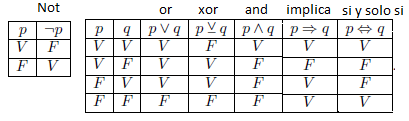
\includegraphics[scale=1]{figuras/tablasDeVerdad/img1.png}
\end{figure}
Los conectores lógicos coinciden con las definiciones de las tablas de operaciones de conjuntos. Teniendo en cuenta que dados dos conjuntos A y B contenidos en un conjunto referencial U nuestras proposiciones  serian algo como:
\begin{equation}
	\left[
	\begin{array}{ccc}
		p: (x \in A)  & y & q : (x \in B) \\
	\end{array}
\right]
\end{equation}


Estas proposiciones así definidas tienen 4 posibilidades de verasidad para cualquier $x \in U$

Vemos, que las operaciones se reducen a las siguientes analogías respercto de las tablas de verdad para conectores lógicos :
\begin{enumerate}
	\item Complemento:  Se corresponde con el \textbf{NOT}
	\item Unión:  La unión entre dos conjuntos se corresponde con el \textbf{OR}
	\item Intersección :  Se corresponde con un \textbf{AND}
	\item Diferencia Simétrica:  Se corresponde con un \textbf{XOR}
	\item Inclusión :  Se corresponde con la \textbf{implicación}
	\item Igualdad:  Se corresponde con un \textbf{si y solo si}. 
	\item Diferencia: $A - B$ se obtiene de la definición $A-B =  A \cap B^c$
\end{enumerate}

\begin{center}
\subsection{Producto Cartesiano} 
\end{center}

\begin{defi}(Producto Cartesiano)
Sean A, B conjuntos. El producto cartesiano de A con B , que se nota
$A X B$ , es el conjunto de pares ordenados:
$$A X B := {(x,y) : x \in A, y \in B}$$
\end{defi}

\newpage

\begin{center}
 \section{Relaciones}
\end{center}

\begin{defi}(Relación)
	Sean A, B conjuntos . Una Relación $\mathcal{R}$ de A en B  es un subconjunto  cualquiera $\mathcal{R}$
del producto cartesiano $A \times B$. Es decir, $\mathcal{R}$ es una relación  de A en B.
\end{defi}

Dados $x \in A$, $y \in B$ y una relación $\mathcal{R}$ de A en B, se dice que \textit{x esta relacionado con y por la relación $\mathcal{R}$}, lo cual lo notamos $x \mathcal{R} y$ y esto se da si $(x,y) \in \mathcal{R}$. Caso contrario la notación es $x \cancel{\mathcal{R}} y$

\begin{center}
\subsection{Relaciones en un conjunto} 
\end{center}

Las relaciones en un conjunto son relaciones de un conjunto en si mismo. 

\begin{defi}(Relación en un conjunto)

	Sea un conjunto A, se dice que $\mathcal{R}$ es una relación en A si: $\mathcal{R} \subseteq A \times A$
\end{defi}	

\begin{defi}(Reflexividad, simetría, antisimetria y transitividad)
Sean un conjunto A  y $\mathcal{R}$ una relación en A, entonces:
\begin{itemize}
	\item \textbf{Reflexividad}: $\mathcal{R}$ se dice \textbf{reflexiva} si $(x,x) \in \mathcal{R}, \forall x \in A$ (Es decir: $x \mathcal{R} x, \forall x \in A$). En grafos es un bucle en el mismo elemento.
	\item \textbf{Simetría}: $\mathcal{R}$ se dice \textbf{simétrica} si: $\forall (x,y) \in A, x \mathcal{R} y \Rightarrow y \mathcal{R} x$. Lo que es la doble flecha entre nodos en un grafo.
	\item \textbf{Antisimetria}: $\mathcal{R}$ se dice \textbf{antisimetrica} si: $\forall (x,y) \in A,  x \mathcal{R} y$ e $y \mathcal{R} x \Rightarrow x = y$
	\item \textbf{Transitividad}: $\mathcal{R}$ se dice \textbf{transitiva} si: $ \forall x,y,z \in A, x \mathcal{R} y $ e $y \mathcal{R} z$ $\Rightarrow  x \mathcal{R} z$
\end{itemize}
\end{defi}

\begin{defi}(Relación de equivalencia y de orden )
Sea A un conjunto y $\mathcal{R}$ una relación en A. 
\begin{itemize}
	\item Relación de equivalencia: Cuando la relacion cumple con ser reflexiva, simetrica y transitiva.
	\item Relación de orden: Cuando la relacion cumple con ser reflexiva, antisimetrica y transitiva.
\end{itemize}
\end{defi}

\begin{defi}(Clase de equivalencia (definición informal))

La clase de equivalencia de $x \in A$ es el subconjunto de $A$ formado por todos los elementos $y$ de $A$ relacionados con $x$, y se nota $\overline{x}$
\end{defi}

\begin{table}[H]
	\begin{tabular}{||c||}
	\hline \\
	\sffamily
	\begin{Large}
		\textbf{\textcolor{B}{Ejemplo de Clase de equivalencia:}}
	\end{Large}
		
	\\\\		
	\sffamily Dado un conjunto $A = \{ 1,2,3,4,5,6,7,8,9,10 \}$, se puede definir la relación de equivalencia ``$\sim$'' talque $x$ x \\ \sffamily  esta relacionado con $y$ ($x \sim y$) si y solo si al dividir $x$ e $y$ por 3 resultan tener ambos elementos el mismo resto. 
	\\\\ Entonces, podemos ver que: \\\\ Si dividimos a $x=1$ por 3 y $y=4$ por 3 
	se obtiene que ambos tienen resto 1, por lo tanto $1 \sim 4$. \\ También que $3 \sim 6$ y que $6 \sim 9$ y por propiedad transitiva, como es una relación de equivalencia $3 \sim 9$,\\ lo cual es cierto ya que todos son múltiplos de 3.  Esto nos permite ``separar'' los números que\\ están relacionados unos con los otros de los que no según la misma relación de equivalencia como sigue:\\ 
			\begin{minipage}[b]{0.4\linewidth}
				\centering
		 		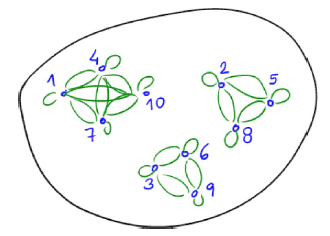
\includegraphics[scale=0.7]{figuras/relaciones/img1.png}
			\end{minipage}	 	
			\begin{minipage}[b]{0.6\linewidth}	
				En la figura se ve claramente que: 
				
				$\overline{1}=\overline{4}=\overline{7}=\overline{10}=\{1,4,7,10\}$
				
				$\overline{2}=\overline{5}=\overline{8}=\{2,5,8\}$
				
				$\overline{3}=\overline{6}=\overline{9}=\{3,6,9\}$
				
				Esto nos da que un conjunto de clases de equivalencia: 
				
				$\{ \overline{1}, \overline{2}, \overline{3}\}$
				
				Siendo estos conjuntos \textbf{Disjuntos dos a dos} o \textbf{Disjuntos por pares}.
				Por lo que, lo que se hizo fue dividir el conjunto $A$ en tres subconjuntos disjuntos entre si 
				cuya únion de dichos conjuntos nos da $A$.				
			\end{minipage}
	\\\\ \hline 		
	\end{tabular}			
\end{table}		

\begin{defi}(Definición formal de Clase de Equivalencia)
Sean $A$ un conjunto y $\sim$ una Relación de equivalencia	 en A. Para cada $	x \in A$, la clase de equivalencia de $x$ es el conjunto:
$$ \overline{x} = \{   y \in A: y \sim x \} \subseteq A$$
\end{defi}

\begin{propo}(Propiedad Fundamental de las clases de equivalencia)
Sean $A$ un conjunto y $\sim$ una Relación de equivalencia	 en A. 
Sean $x,  y \in A$, entonces o bien $\overline{x} \cap \overline{y}$, o bien $\overline{x} = \overline{y}$
\end{propo} 

\begin{propo}(Relaciones de equivalencia y particiones)
Sea $A$ un conjunto. Hay una manera natural de asociarle a una relación de equivalencia en $A$ una partición de $A$. Recíprocamente, a toda partición se le puede asociar una relación de equivalencia y estas asociaciones son inversas una de la otra. 
\end{propo}


\begin{center}
\section{Funciones}
\subsection{¿Que es una función?} 
\end{center}


\begin{defi}(Función)
	Sean $A$ y $B$ conjuntos, y sea $\mathcal{R}$ una relación de $A$ en $B$. Se dice que $\mathcal{R}$ es una función cuando todo elemento  $x \in A$ esta relacionado con algún $y \in B$, y este elemento $y$ es único. Es decir:
	$$\forall x \in A, \, \exists ! \, y\in B: \, x\mathcal{R}y$$
\end{defi}

\begin{obs}
Los elementos del conjunto $A$ (el dominio) deben estar todos relacionados con un elemento del conjunto $B$ (denomindado codiminio). 
Ademas, si un mismo elemento del conjunto $A$ apunta a dos elementos diferentes del conjunto $B$, entonces esta relación no es función. 

Por otro lado, el primer problema puede solucionarse \textit{\textbf{restringiendo el dominio}}. 

\end{obs}


\begin{defi}(Igualdad de Funciones)
Sean $f, \, g: A \rightarrow B$ funciones. Se tiene:
	$$f = g \, \Leftrightarrow \, f(x) = g(x), \forall x \in A$$
\end{defi}

\begin{defi}(Imagen)
Sea $\! f: A \rightarrow B$ función. La \textbf{imagen} de $f$, que se nota $Im(\! f)$, es el  subconjunto de elementos de $B$ que estan relacionados con algún elemento de $A$. Es decir:
$$Im(f) = \{ y \in B: \exists x \in A \, tal que \, f(x)=y \}$$
\end{defi}

\begin{center}
\subsection{Funciónes inyectivas, sobreyectivas y biyectivas} 
\end{center}

\begin{defi}(Funciones Inyectivas, sobreyectivas y biyectivas)
Sea $f: A \rightarrow B$ una función. Se dice que:
\begin{itemize}
	\item $f$ es \textbf{inyectiva} si para todo elemento $y \in B$ existe a lo sumo un elemneto $x \in A$ para el cual $f(x)=y$. Dicho de otra forma, $f$ es inyectiva si para todo $x, x' \, \in A$ tales que $f(x) = f(x')$ se tiene que $x = x'$.
	\item $f$ es \textbf{sobreyectiva} si para todo elemento $y \in B$ existe al menos un elemento $x \in A$ para el cual $f(x) = y$. Dicho de otra manera, $f$ es sobreyectiva si $Im(f) = B$.
	\item $f$ es \textbf{biyectiva} si es a la vez inyectiva y sobreyectiva, es decir para todo elemento $y \in B$ existe exactamente un elemento $x \in A$ para el cual $f(x) = y$.
\end{itemize} 
\end{defi}

\begin{defi}(Composición de funciones)
Sean $A$, $B$, $C$ conjuntos, y $f: A \rightarrow B$, $g: B \rightarrow C$ funciones. Entonces la composición de $f$ con $g$, que se nota $g \circ f$, definida por  
$$g \circ f(x) = g\left( f(x)\right), \forall x \in A$$
\end{defi}

\begin{defi}(Función inversa)
Sea $f : A \rightarrow B$ biyectiva, entonces $f^{-1} : B \rightarrow A$ se llama \textbf{función inversa} y es una función que satisface que $\forall y \in B \, f^{-1}(y)=x \, \Leftrightarrow \, f(x)=y$
\end{defi}
\begin{propo}(Biyectividad y Función inversa)
Sea $f : A \rightarrow B$ una función:
\begin{itemize}
	\item Si $f$ es biyectiva, entonces $f^{-1} \circ f = id_{A}$ y $f \circ f^{-1} = id_{B}$
	\item Si existe una función $g : B \rightarrow A$ tal que $g \circ f = id_{A}$ y  $f \circ g = id_{B}$
	Entonces $f$ es biyectiva y $f^{-1} = g$
\end{itemize}
\end{propo}

\begin{center}
 \section{Números Naturales}
 \subsection{¿Qué son los números naturales ($\mathbb{N}$)?}
\end{center}

Los naturales son, informalmente el conjunto:
$$\mathbb{N} = \{1,2,3, \cdots , 1001, 1002, \cdots, \}$$
En este conjunto se puede sumar y multiplicar (No existen los numeros negativos):
$$si \, m,n \in \mathbb{N} \Rightarrow m+n \in \mathbb{N} \, \land \, m \cdot n \in \mathbb{N}$$
Propiedades que se satisfacen en este conjunto de números son:
\begin{itemize}
	\item Conmutatividad: $m+n = n+m$ y $m \cdot n = n \cdot m$ $\forall \, m,n \in \mathbb{N}$
	\item Asociatividad:
	\item Distributividad del producto sobre la suma:
\end{itemize}

\begin{center}
 \subsection{La suma de Gauss y la serie Geométrica}
\end{center}

\subsubsection{La suma de Gauss}
Supongamos que queremos sumar una cierta cantidad $n$ de números, de manera que:
$$r = 1+2+3+4 + \cdots + n $$
Este procedimiento se puede generalizar como sigue:
$$\forall \, n\in \mathbb{N}: \, 1+2+3+ \cdots + (n-1) + n = \frac{n(n+1)}{2}$$
Notar que este siempre sera un numero natural y que $n(n+1)$ siempre es un numero \textbf{par}.
\subsubsection{La serie Geométrica}
Sea un número $q$ cualquiera, queremos sumar las $n + 1$ primeras potencias de $q$:
$$1+q+q^2+\cdots+q^{n-1}+q^n$$
Esto resulta en:
\begin{displaymath}
\forall n \in \mathbb{N}: \, 1+q+ \cdots + q^n = \left\{ \begin{array}{cc}
 n+1 & \mbox{si \, q=1}   \\
		\! \frac{q^{n+1} - 1}{q-1} & \mbox{si \, q \cancel{=} 1}  \\
 \end{array}\right.
\end{displaymath}

\begin{center}
 \subsection{Sumatoria }
\end{center}

\begin{defi}(Sumatoria)
	Sea $n \in \mathbb{N}$. La notación $ \displaystyle\sum^{n}_{i=1} a_i $ que se lee \textbf{la sumatoria para $i$ de 1 a n de $a_i$}, la cual representa la suma de los primeros $n$ términos de la sucesión $(a_i)_{i \in \mathbb{N}}$:
	$$ \displaystyle\sum^{n}_{i=1} a_i = a_1 + \cdots + a_n$$
	La cual por recurrencia se define de la siguiente forma:
	$$ \displaystyle\sum^{1}_{i=1} a_i = a_1 \,\ \,\ y \,\ \,\ \displaystyle\sum^{n+1}_{i=1} a_i = a_i + a_{n+1} \, , \, \forall n \in \mathbb{N}$$
\end{defi}

\begin{prop}(Propiedades de sumatorias)
\begin{itemize}
	\item $\left( \displaystyle\sum^{n}_{i=1} a_i \right) + \left( \displaystyle\sum^{n}_{i=1} b_i \right) =  \displaystyle\sum^{n}_{i=1} (a_i + b_i)$ 
	\item  $ c \cdot \displaystyle\sum^{n}_{i=1} a_i = \displaystyle\sum^{n}_{i=1} c \cdot a_i$
\end{itemize}
\end{prop}

\begin{center}
 \subsection{Productoria}
\end{center}

\begin{defi}
Sea $n \in \mathbb{N}$. La notación $\displaystyle \prod_{i=1}^{n} a_i$, que se lee \textbf{la productoria para $i$ de 1 a $n$ de $a_i$}, representa el producto de los $n$ primeros términos de la sucesión $(a_i)_{i \in \mathbb{N}}$:
$$\displaystyle \prod_{i=1}^{n} a_i = a_1 \cdots a_n$$
Siendo por recursión:
$$\displaystyle \prod_{i=1}^{1} a_i = a_1 \, y \displaystyle \prod_{i=1}^{n+1} a_i = \left( \displaystyle \prod_{i=1}^{n} a_i \right) \cdot a_{n+1} \, , \, \forall n \in \mathbb{N}$$
\end{defi}
\begin{prop}(Propiedad de la productoria)
$$\left( \displaystyle \prod_{i=1}^{n} a_i \right) \cdot \left( \displaystyle \prod_{i=1}^{n} b_i \right) =  \displaystyle \prod_{i=1}^{n} (a_i \cdot b_i)$$
\end{prop}

\begin{center}
 \subsection{El conjunto inductivo $\mathbb{N}$ y el principio de inducción}
\end{center}

\begin{defi}(Conjunto Inductivo)
Sea $\mathbf{H} \subseteq \mathbb{R}$  un conjunto.  Se dice que $\mathbf{H}$ es un conjunto inductivo si se cumplen las dos condiciónes siguientes:
\begin{itemize}
	\item $1 \in \mathbf{H}$
	\item $\forall x, \, x \in \mathbf{H} \Rightarrow x + 1 \in \mathbf{H}$ 
\end{itemize}
\end{defi}

\begin{teo}(Principio de Inducción)

Sea $p(n), \, n \in \mathbb{N}$, una afirmación sobre los numeros naturales. Si $p$ satisface
\begin{itemize}
	\item Caso Base: $p(1)$ es \textit{verdadera}
	\item Paso Inductivo: $\forall h \in \mathbb{N}, \, p(h)$ Verdadera $\Rightarrow \, p(h+1)$ Verdadera
\end{itemize}
Entonces, $p(n)$ es Verdadero, $\forall n \in \mathbb{N}$(h := Hipotesis $\Rightarrow$ $p(h) :=$ Hipotesis Inductiva (HI)) 
\end{teo}

\begin{teo}(Principio de Induccion Corrido)
Sea $n_0 \in \mathbb{Z}$ y sea $p(n), \, n \leq n_0$, una afirmación sobre $\mathbb{Z}_{n_0}$. Si $p$ satisface :
\begin{itemize}
	\item Caso Base: $p(n_0)$ es Verdadera
	\item Paso Inductivo: $\forall h \leq n_0$, $p(h)$ Es Verdadera $\Rightarrow \, p(h+1)$ esVerdadera y entonces $p(n)$ es Verdadera $\forall n \in \mathbb{N}$
\end{itemize}
\end{teo}

\begin{center}
 \subsection{Inducción Completa}
\end{center}

\fbox{\begin{minipage}[b][1.7\height]%
[t]{0.5\textwidth} 
\begin{teo}(Princiío de inducción - $\mathbf{II}$)

Sea $p(n), \, n \in \mathbb{N}$, una afirmación sobre los números naturales. Si $p$ satisface
\begin{itemize}
	\item Caso Base: $p(1)$ y $p(2)$ son Verdaderas
	\item Paso Inductivo: $\forall h \in \mathbb{N}, \, p(h) \, y \,  p(h + 1) \, Verdaderas \, \Rightarrow p(h+2) \, Verdadera$
\end{itemize}
entonces, $p(n)$ es verdadera, $\forall n \in \mathbb{N}$
\end{teo}
\end{minipage}}
\fbox{\begin{minipage}[b][1.7\height]%
[t]{0.5\textwidth} 
\begin{teo}(Princiío de inducción - $\mathbf{II}$ corrido)

Sea $n_0 \in \mathbb{Z}$ y sea $  p(n)  n \leq n_0$, una afirmación sobre los $\mathbb{Z}_{\leq n_0}$.
Si $p$ satisface:
\begin{itemize}
	\item i Base: $p(n_0)$ y $p(n_0 + 1)$ son Verdaderas
	\item Paso Inductivo: $\forall h \leq n_0, \, p(h) \, y \,  p(h + 1) \, Verdaderas \, \Rightarrow p(h+2) \, Verdadera$
\end{itemize}
entonces, $p(n)$ es verdadera, $\forall n \in \leq n_0$
\end{teo}
\end{minipage}}

\newpage
\begin{center}
 \subsection{Sucesión de Fibonacci}
\end{center}

Fibonacci presento el siguiente problema: Imaginemos que colocamos una pareja de conejos bebes en un área cerrada ¿Cuantos conejos habra despues de $n$ meses si:
\begin{enumerate}
\item Los conejos nunca mueren.
\item Cada pareja de conejos produce una nueva pareja de conejos cada mes
\item Comienzan a tener parejitas luego de dos meses de nacida
\end{enumerate}

Dadas estas condiciones se obtiene la sucesión de Fibonacci $(F_{n})_{n \in \mathbb{N}_0}$:
$$ F_0 = 0, \, F_1 = 1 \, \, F_{n+2} = F_{n+1} + F_n \, , \, \forall n \in \mathbb{N}_0$$

\fbox{\begin{minipage}[b][1.2\height]%
[t]{0.7\textwidth} 
\begin{propo}(Termino General de la Sucesión de Fibonacci)
$$F_n = \frac{1}{\sqrt{5}}(\phi^n - \overline{\phi^n})$$
Donde: $$\phi = \frac{1 + \sqrt{5}}{2} \simeq 1,61803 \hspace{0.3cm} \land \hspace{0.3cm} \overline{\phi} = \frac{1 -\sqrt{5}}{2} < 0$$
\end{propo}
\end{minipage}}

\begin{center}
 \subsection{Sucesión de Lucas}
\end{center}

Una sucesión de Lucas es una sucesión $(a_n)_{n \in \mathbb{N}_0}$ definida recursivamente por:
$$a_0 = a, \, a_1 = b, \, \, a_{n+2} = c a_{n+1} + d a_n, \, \forall n \in \mathbb{N}_0$$
Con $a, \, b, \, c, \, d, \, \in \mathbb{C}$ 

Si consideramos la ecuación $\mathbf{X}^2 - c \mathbf{X} - d=0$ asociada a la sucesión $(a_n)_{n \in \mathbb{N}_0}$. Suponiendo que esta tiene dos raíces, tales que:
$$r^2 = c r + d \, y \, \overline{r}^2 = c \overline{r} + d$$
Se dan las siguientes afirmaciones:
\begin{enumerate}
 \item Las sucesiones $(r^n)_{n \in \mathbb{N}_0}$, $(\overline{r}^n)_{n \in \mathbb{N}_0}$ y cualquier combinación de la forma:
 $$(\lambda_n)_{n \in \mathbb{N}_0} = (\alpha r^n + \beta \overline{r}^n)_{n \in \mathbb{N}_0}$$
 Satisfacen la misma recurrencia que la sucesión de Lucas $(a_n)_{n \in \mathbb{N}_0}$  siendo la recurrencia la siguiente:
 $$\lambda_{n+2} = c \lambda_{n+1} + d \lambda_n \, , \, \forall n \in \mathbb{N}$$
 \item $\exists ! (\lambda_n)_{n \in \mathbb{N}_0} = (\alpha r^n + \beta \overline{r}^n)_{n \in \mathbb{N}_0}$ que satisface las \textbf{condiciones iniciales} $\lambda_0 = a \, , \, \lambda_1 = b$
 
 Resultado del cual sale de resolver:
 \begin{displaymath}
 	\left\{ \begin{array}{ccc}
 		\alpha + \beta = a & \Rightarrow & \alpha = \cfrac{b - a \overline{r}}{r - \overline{r}} \\
 		\alpha r + \beta \overline{r} = b & \Rightarrow & \beta = \cfrac{a r - b}{r - \overline{r}}
 	\end{array}\right.
 \end{displaymath}
 Concluyendo que $(a_n)_{n \in \mathbb{N}_0} = (\lambda_n)_{n \in \mathbb{N}_0} = (\alpha r^n + \beta \overline{r}^n)_{n \in \mathbb{N}_0}$
 \item Dada la ecuación asociada $\mathbf{X}^2 - c \mathbf{X} - d=0$ con solo una raíz ($\mathbf{X}^2 - c \mathbf{X} - d= (\mathbf{X} - r)^2$ ). En este caso, las sucesiónes $(r^n)_{n \in \mathbb{N}_0}$ y $( n r^{n-1})_{n \in \mathbb{N}_0}$ satisfacen la misma recurrencia y tamien cualquier combinación lineal con \textbf{las condiciones iniciales}  $\lambda_0 = a \, , \, \lambda_1 = b$, se tiene que el termino general para $a_n$ cuando $r \cancel{=} 0$, es:
 $$a_n = a r^n + (b -a r)n r^{n-1} \, , \, \forall n \in \mathbb{N}_0 $$
\end{enumerate}
 
 \begin{center}
  \subsection{Inducción Completa}
 \end{center}

 \begin{teo}(Principio de Inducción Completa)
Sea $p(n)$, $n \in \mathbb{N}$ una afirmación en los numeros naturales. Si $p$ satisface:
\begin{itemize}
	\item Caso Base:  p(1) es Verdadera
	\item Paso Inductivo: $\forall \, h \in \mathbb{N}, \, p(1) \cdots p(h)$ es Verdadera $\Rightarrow$ $p(h +1)$ es verdadera
\end{itemize}
entonces $p(n)$ es Verdadera, $\forall n \in \mathbb{N}$
\end{teo}


\newpage
\begin{center}
 \section{Combinatoria}
 \subsection{Cardinal}
\end{center}

\begin{defi}(Cardinal)

Dado el conjunto $A$, el cardinal de $A$ ($\# A$) a la cantidad de elementos \textit{distintos} que tiene $A$.
\end{defi}

\begin{obs}(Cardinal de un Subconjunto)

Sea $A$ un conjunto finito y $B \subseteq A$, entonces $\# B \leq \# A$
\end{obs}

\begin{prop}(Cardinales de Union, Interseccion, Complemento y otros)
	
	
	\begin{enumerate}
		\item $A$ $\land$ $B$ conjuntos disjuntos (\textit{sin ningun elemento en comun}), entonces: $\#(A \cup B) = \# A + \# B$
		\item Si $A$ $\land$ $B$ no son disjuntos (\textit{tienen al menos un elemento en comun}), enconces:  $\#(A \cup B) = \# A + \# B - \#(A \cap B)$
		\item Si $U$ es un conjunto finito, entonces: $\#(A^c) = \# U - \# A$
		\item $\#(A-B) = \#A - \#(A \cap B)$
		\item $\#(A \vartriangle B) = \# A + \# B - 2 \#(A \cap B)$
		\item $\#(A x B) = \#A \cdot \#B$
		\item $\#(\mathcal{P}(A)) = 2^{\#A}$
		\item $\# (A^n) = (\# A^n)$
		
	\end{enumerate}
\end{prop}

\begin{center}
\subsection{Cantidad de relaciones y funciones} 
\end{center}

\begin{prop}(Cantidad de Relaciones)

Sean $A_m$ y $B_n$ conjuntos finitos, con $m$ y $n$ elementos respectivamente. Entonces, la cantidad de relaciones que hay de $A_m$ en $B_m$ es igual a $2^{mn}$
\end{prop}

\begin{prop}(Cantidad de Funciones)

Sean $A_m$ y $B_n$ conjuntos finitos, con $m$ y $n$ elementos respectivamente. Entonces, la cantidad de funciones que hay de $A_m$ en $B_m$ ($\# (f: A \rightarrow B)$) es igual a $n^m$.
\end{prop}

\begin{prop}(Cardinal de Conjuntos y Funciones)

Sean $A$ y $B$ Conjuntos finitos:
\begin{itemize}
	\item $f: A \rightarrow B$ inyectiva $\implica$ $\# A \menig \# B$
	\item $f: A \rightarrow B$ sobreyectiva $\implica$ $\# A \mayig \# B$
	\item $f: A \rightarrow B$ biyectiva $\implica$ $\# A = \# B$
\end{itemize}
\end{prop}


\begin{defi}(Cantidad de Funciones Inyectivas )

Sean $A_m$ y $B_n$ conjuntos finitos, con $m$ y $n$ elementos respectivamente, donde $m \menig n$. Entonces, la cantidad de funciones inyectivas de $f: A_m \rightarrow B_n$ que hay son:
\[n \cdot (n-1) \cdots (n-m+1) = \frac{n!}{(n-m)!}\]
\end{defi}

\begin{defi}(Cantidad de Biyecciones (Permutaciones))

Sea $n \in \mathbb{N}$. La cantidad de funciones biyectivas que hay entre dos conjuntos de $n$ elementos o cantidad de permutaciones esta dado por el factorial de los $n$ elementos de los conjuntos:
\[\#(f: A_n \rightarrow B_n) = n! = n \cdot (n-1) \cdots 2 \cdot 1 = \prod_{i=1}^n i\]
Definicion por recurrencia del factorial:
\[0!=1 \hspace{0.5cm} \land \hspace{0.5cm} n! = n \cdot (n-1)! ,\hspace{0.5cm} \forall n \in \mathbb{N}\]
\end{defi}

\begin{teo}(Numero Combinatorio)

Sean $n \in \mathbb{N}$ y sea $A_n$ un conjunto de $n$ elementos. Para $0 \menig k \menig n$, la cantidad de subconjuntos con $k$ elementos del conjunto $A_n$ 
\[\comb{n}{k} = \frac{n!}{k!(n-k)!}\]
\small{\texttt{(Formas de elegir $k$ elementos de un conjunto de $n$)}}
\end{teo}

\begin{obs}(Recordar)

\begin{itemize}
\item $\comb{n}{0} = \comb{n}{n} = 1$
\item $\comb{n}{1} = \comb{n}{n-1} = n$
\item $\comb{n}{k} = \comb{n}{n-k} $
\item $2^n = \sum_{k=0}^{n} \comb{n}{k}$
\end{itemize}
\end{obs}

\begin{teo}(Binomio de Newton)
\[(x-y)^n = \sum_{k=0}^{n} \comb{n}{k} x^k y^{n-k} , \hspace{0.2cm} \forall n \in \mathbb{N}_0\]
\end{teo}


\begin{center}
\section{Enteros}
\subsection{Divisibilidad} 
\end{center}

\begin{defi}{Divisivilidad}
Sean $a,d \in \entero{}$ con $d \neq 0 $. Se dice que $d$ divide a $a$ y se nota $d|a$ si se cumple:
\[d|a \sii \exists k \in \entero : a = k \cdot d\]
\end{defi}

\begin{prop}{De la divisibilidad} 
\begin{itemize}
 \item[   (i)] $d \neq 0$ $\implica$ $d | 0$, pues $k = 0$ cumple $0 = k \cdot d$
 \item[  (ii)] $d | a$ $\sii$ $- d | a$. Se concluye $d | a$ $\sii$ 
 $|d| \left\vert \right. |a|$ 
 \item[ (iii)] $a \neq 0$, $d|a$ $\implica$ $|d| \menig |a|$
 \item[  (iv)] Los únicos inversibles en $\entero{}$ son el $1$ y el $-1$.
 \item[   (v)] $d|a$ y $a|d$ $\sii$ $a = \pm d$
 \item[  (vi)] $d|a$ y $d|b$ $\implica$ $d|a+b$ (no vale la vuelta)
 \item[ (vii)] $d|a$ y $d|b$ $\implica$ $d|a-b$ (no vale la vuelta)
 \item[(viii)] $d|a$ $c \in \entero{}$ $\implica$ $d|c \cdot b$
 \item[  (ix)] $d|a$ $\implica$ $d^n|a^n$, $\forall n \in \natural{}$
 \item[   (x)] $d|a\cdot b$ $\not\implica$ $d|a$ y $d| b$ (esto solo se cumplira cuando $d$ es primo) 
\end{itemize}
\end{prop}

\begin{defi}{Primos y Compuestos}
 Se dice que $a \in \entero{}$ es un número $primo$ si $a \neq 0, \pm 1$ y tiene unicamente $4$ divisores $(\pm 1 , \pm a)$.
 
 Luego, se dice $compuesto$ cuando no es primo
\end{defi}

\begin{center}
\subsection{Congruencia} 
\end{center}


\begin{defi}{Congruencia}
 Sea $d \in \entero{}$, $d \neq 0$. Dados $a,b \in \entero{}$, se dice que $a$ es congruente a $b$ modulo $d$ si se tiene que $d | a - b$
 \[\congruente{a}{b}{d} \sii \hspace{0.3cm}  \divi{d}{a - b} \]
\end{defi}

\begin{propo}{La congruencia es una relacion de equivalencia}
 Sea $d \in \entero{}$, $d \neq 0$. Sea $\mathcal{R}$ la relación en $\entero{}$ dada por:
 \[a \mathcal{R} b \sii \congruente{a}{b}{d} ,\hspace{0.3cm}\forall a,b \in \entero{}\]
Entonces $\mathcal{R}$ es relación de equivalencia.
 \end{propo}

\begin{prop}{De la congruencia}
Sea $d \in \entero{}$, $d \neq 0$. Entonces:
\begin{enumerate}
 \item $\forall$ $a_1,a_2,b_1,b_2 \in \entero{}$
 \[\congruente{a_1}{b_1}{d} \es{0.2} y \es{0.2} \congruente{a_2}{b_2}{d} \es{0.2} \implica \es{0.2} 
 \congruente{a_1 +a_2}{b_1+b_2}{d}\]
 \item $\forall$ $a, b, c \in \entero{}$
 \[\congruente{a}{b}{d} \es{0.2} \implica \es{0.2} \congruente{c a}{c b}{d}\]
 \item $\forall$ $a_1,a_2,b_1,b_2 \in \entero{}$
 \[\congruente{a_1}{b_1}{d} \es{0.2} y \es{0.2} \congruente{a_2}{b_2}{d} \es{0.2} \implica \es{0.2} 
 \congruente{a_1 a_2}{b_1 b_2}{d}\]
 \item $\forall$ $a, b\in \entero{}$ y $n \in natural{}$
 \[\congruente{a}{b}{d} \es{0.2} \implica \es{0.2} \congruente{a^n}{b^n}{d}\]
\end{enumerate}
\end{prop}

\begin{center}
    \subsection{Algoritmo de División} 
\end{center}


\begin{teo}{Algoritmo de División}
Dados, $a,d \in \entero{}$ con $d \neq 0$,  $k,r \in \entero{}$ que satisfacen:
\[a = k \cdot d + r \es{0.2} con \es{0.2} 0 \menig r < d \]
A $k$ se le da el nombre de conciente y a $r$ el nombre de resto.
\end{teo}

\begin{obs}{}
 Si $ 0 \menig a < |d| $, entonces $a = 0 \cdot d + a$ implica que $k = 0$ y el resto $r = r_d(a)=a$, pues $a$ cumple la condicion que tiene que cumplir el resto (se aplica la unicidad del cociente y el resto).
\end{obs}

\begin{obs}{Divisibilidad y Resto}
Sean $a, d \in entero{}$, $d \neq 0$. Entonces:
\[r_d(a)= 0  \es{0.2} \sii \es{0.2} \divi{d}{a} \es{0.2} \sii \es{0.2} \congruente{a}{0}{d}\]
\end{obs}

\begin{prop}{Congruencia y Resto}
Sea $d \in entero{}$, $d \neq 0$. Entonces:
\begin{itemize}
 \item[($\alpha$)] $\congruente{a}{r_d(a)}{mod \es{0.1} d}$, $\forall a \in \entero{}$ 
 \item[ ($\beta$)] $\congruente{a}{r}{mod \es{0.1} d}$ con $0 \menig r < d$, entonces $r = r_d(a)$
 \item[($\gamma$)] $\congruente{r_1}{r_2}{d}$ con $0 \menig r_1, r_2 < d$, entonces $r_1 = r_2$
 \item[($\delta$)] $\congruente{a}{b}{d}$ $\sii$ $r_d(a) = r_d(b)$
\end{itemize}
\end{prop}

\begin{cor}{Tablas de Restos}
 Sean $a,b,d \in \entero{}$, $d \neq 0$. Entonces:
 \begin{itemize}
  \item $r_d(a+b) = r_d(r_d(a)+r_d(b))$
  \item $r_d(a\cdot b) = r_d(r_d(a) \cdot r_d(b))$
  \item $r_d(a^n) = r_d(r_d(a^n))$
 \end{itemize}
\end{cor}

\begin{center}
\subsection{Maximo Comun Divisor} 
\end{center}

\begin{defi}{Maximo Común Divisor}
Sean $a,b \in \entero{}$, no ambos nulos. El \rojo{maximo comun divisor (mcd)} entre $a$ y $b$, se nota $(a:b)$, es el mayor de los divisores comunes de $a$ y  $b$. Es decir:
\[(a:b) | a, \es{0.1} (a:b) | b \es{0.2} y \es{0.1} si \es{0.2} \divi{d}{a} \es{0.2} y \es{0.2} \divi{d}{b} \es{0.2} \implica \es{0.2} d \menig (a:b)\]
\end{defi}

\begin{propo}{}
 Sean $a, b \in \entero{}$ no ambos nulos, y sea $k \in \entero{}$, entonces:
 \[DivCom(\{a,b\})   =  DivCom(\{b,a - k \cdot b\})\]
 \[DivCom_+(\{a,b\}) =  DivCom(\{b,a - k \cdot b\})\]
 En particular, $\forall k \in \entero{}$, $(a:b) = (b,a - k \cdot b)$
 
 Aplicando esto a $r_b(a) = a - k\cdot b$, se obtiene que $(a:b) = (b,r_b(a))$
\end{propo}

\begin{teo}{Algoritmo de Euclides}
Sean $a, b \in \entero{}$ no ambos nulos. Existe $l \in \natural{}$ tal que en una sucesión finita de $l+1$ divisiones:
\begin{center}
$a = k_1 \cdot b + r_1     \es{0.3} con \es{0.2} 0 \menig r   < |b|$

$b = k_2 \cdot r_1 + r_2   \es{0.3} con \es{0.2} 0 \menig r_2 < r_1$ 

$r_1 = k_3 \cdot r_2 + r_3 \es{0.3} con \es{0.2} 0 \menig r_3 < r_2$
.

.

.

$r_{l-2} = k_l \cdot r_{l-1} + r_l \es{0.3} con \es{0.2} 0 \menig r_l < r_{l-1}$

$r_{l-1} = k_{l+1} \cdot r_{l} + r_{l+1} \es{0.3} con \es{0.2} 0 \menig r_{l+1} < r_{l}$
\end{center}
Se llega por primera vez al resto nulo $r_{l+1}$. Entonces $(a:b)=r_l$, el ultimo resto no nulo. 
\end{teo}

\begin{obs}{}
 Si $a, b \in \entero{}$ son tales que $a=0$ y $b \neq 0$, ya sabemos que $(a:b) = |b|$. Por lo tanto, el Algoritmo de Euclides permite calcular el mcd de aualquier par de $\entero{}$ no ambos nulos.
\end{obs}

\begin{teo}{MCD y Combinación Entera}
 Sean $a, b \in \entero{}$, no ambos nulos. Entonces existen $s, t \in \entero{}$ tales que:
 \[(a:b) = s \cdot a + t \cdot b\]
\end{teo}

\begin{obs}{Combinaciones enteras de $a$ y $b$}
Si $a, b \in \entero{}$ no ambos nulos, y $c \in \entero{}$.
\begin{center}
 $c = s' \cdot a + t' \cdot b$ para $s', t' \in \entero{}$ $\sii$ $(a:b) = c$
\end{center}
\end{obs}

\begin{propo}{MCD y Divisores Comunes}
Si $a, b \in \entero{}$ no ambos nulos,  y sea $d \in \entero{}$, con $d \neq 0$. Entonces
\[\divi{d}{a} \es{0.2} y \es{0.2} \divi{d}{b} \es{0.3} \sii \es{0.3} \divi{d}{(a:b)}\]
\end{propo}

\begin{propo}{MCD de múltiplo comun de dos números}
 Si $a, b \in \entero{}$ no ambos nulos, y sea $k \in \entero{} / \{0\}$. Entonces:
 \[(k \cdot a : k \cdot b) = |k| (a:b)\]
\end{propo}

\begin{teo}{Equivalencias del mcd}
 Si $a, b \in \entero{}$ no ambos nulos,  y sea $d \in \natural{}$. Son equivalentes:
 \begin{enumerate}
  \item $\divi{d}{a}$, $\divi{d}{b}$ y si $\divi{c}{a}$ y $\divi{c}{b}$, entonces $c \menig d$
  \item $\divi{d}{a}$, $\divi{d}{b}$ y existen $s, t \in \entero{}$ tales que 
  $d = s a + t b$
  \item $\divi{d}{a}$, $\divi{d}{b}$ y si $\divi{c}{b}$, entonces $\divi{c}{d}$
 \end{enumerate}
Un numero $d \in \nat{}$ que cumple cualquiera de esas $3$ propiedades es el máximo comun divisor $(a:b)$.
\end{teo}


\begin{center}
\subsection{Números Coprimos} 
\end{center}


\begin{defi}{Números Coprimos}
 Se dice que $a,b \in \entero{}$ no ambos nulos son coprimos, si y solo si $(a:b)=1$. Es decir, si y solo si los únicos divisores comunes de $a$ y $b$ son $\pm 1$.
\end{defi}

\begin{obs}{Coprimos y Combinación Entera}
 Sean $a,b \in \entero{}$ no ambos nulos. Entonces
 \[ (a:b)=1 \es{0.3} \sii \es{0.3} \exists \es{0.1} s,t \in \entero{}\es{0.1} :\es{0.1} 1 = s a + t b\]
\end{obs}

\begin{prop}{Escenciales de divisibilidad con coprimalidad}
Sean $a,b,c,d \in \entero{}$ con $c \neq 0$ y $d \neq 0$. Entonces
 
\begin{enumerate}
 \item $\divi{c}{a}$, $\divi{d}{a}$ y $(c:d)=1$ $\implica$ $\divi{c d}{a}$
 \item $\divi{d}{a b}$ y $(d:a)=1$ $\implica$ $\divi{d}{b}$
\end{enumerate}
\end{prop}

\begin{propo}{Coprimizando}
 Sean $a,b \in \entero{}$ no ambos nulos. Entonces:
 \[\left(\frac{a}{(a:b)} : \frac{b}{(a:b)}\right) = 1\]
 Por lo tanto
 \[a = (a:b)a' \es{0.2} b = (a:b)b'\]
 Donde los numeros $a' = \frac{a}{(a:b)}$ y $b' = \frac{b}{(a:b)}$ son coprimos.
\end{propo}

\begin{center}
\subsection{Primos y Factorización}   
\end{center}

\begin{propo}{Todo número entero distindo de 0 y  1 es divisible por algún primo}
 Sea $a \in \entero{}$, $a \neq 0, \pm 1$. Entonces, existe un numero primo positivo $p$, tal que $\divi{p}{a}$
\end{propo}

\begin{cor}{Cantidad de Primos}
Existen infinitos primos positivos distintos.
\end{cor}

\begin{teo}{Propiedad Funcamental de los números primos}
 Sea $p$ un primo y sean $a,b \in \entero{}$. Entonces:
 \[\divi{p}{a \cdot b} \es{0.2} \divi{p}{a} \es{0.2} o \es{0.2} \divi{p}{b}\]
\end{teo}

\begin{propo}{}
 Sea $p$ un número primo y sean $a_1, \cdots, a_n \in \entero{}$, con $n \mayig2$. Entonces:
 \[\divi{p}{a_1} \cdots c_n \es{0.2} \implica \es{0.2} \divi{p}{a_i}\es{0.2} para \es{0.1} algun \es{0.1} i, \es{0.2} 1 \menig i \menig n\]
 En particular, dado $a \in \entero{}$, si $\divi{p}{a^n}$ entonces $\divi{p}{a}$
\end{propo}

\begin{teo}{Teorema fundamental de la Aritmetica}
 Sea $a \in \entero{}$, $a \neq 0, \pm 1$. Entonces $a$ se escribe en forma única como pŕoducto de primos positivos (factorización única), es decir:
 \[a = \pm p_1^{m_1} \cdot \pm p_1^{m_1} \cdots \pm p_r^{m_r} \]
 Esta escritura es única salvo permutación de primos.
\end{teo}

\begin{obs}{Primos de productos y potencias}
Sean $a,b \in \entero{}$ no nulos de la forma 
\begin{center}
 $a = \pm p_1^{m_1} \cdot \pm p_2^{m_2} \cdots \pm p_r^{m_r}$, con $m_i \in \nat{}_0$
 $b = \pm p_1^{n_1} \cdot \pm p_2^{n_2} \cdots \pm p_r^{n_r}$, con $n_i \in \nat{}_0$
 \end{center}
 Entonces:
 \begin{itemize}
  \item $a \cdot b = (\pm p_1^{m_1}  \cdots \pm p_r^{m_r}) \cdot (\pm p_1^{b_1}  \cdots \pm p_r^{n_r}) = \pm p_1^{m_1 + n_1}  \cdots \pm p_r^{m_r + n_r}$
  
  Es decir, $a \cdot b$ tiene exactamente los primos de $a$ y $b$ en su factorización y los exponentes se suman.
  \item $a^n = (\pm p_1^{m_1}  \cdots \pm p_r^{m_r})^n = (\pm 1)^n \cdot \pm p_1^{m_1 n}  \cdots \pm p_r^{m_r n}$
  
  Es decir, $a^n$ tiene exactamente los mismos primos que $a$ en su factorización y los exponentes van multiplicados por $n$.
 \end{itemize}
\end{obs}

\begin{propo}{Divisores de un número y cantidad}
 Sea $a \in \entero{}$, $a \neq 0 \pm 1$, y sea $a = \pm p_1^{m_1} \cdots p_r^{m_r}$ la factorización en primos de $a$. Entonces
 \begin{enumerate}
  \item $\divi{d}{a}$ $\sii$ $d = \pm p_1^{n_1} \cdots p_r^{n_r}$ con $0 \menig n_i \menig m_i$
  \item $\# Div_+(a) = (m_1 + 1) \cdots (m_r + 1)$ y $\# Div(a) =2 (m_1 + 1) \cdots (m_r + 1)$ 
 \end{enumerate}
\end{propo}

\begin{propo}{Divisores y Potencias}
 Sean $a,d \in \entero{}$ con $d$ no nulo, y sea $n \in \nat{}$. Entonces:
 \[\divi{d}{a} \sii \divi{d^n}{a^n}\]
\end{propo}

\begin{propo}{MCD y factorización}
Sean $a, b \in \entero{}$ no nulos de la forma:
\begin{center}
 $a = \pm p_1^{m_1} \cdot \pm p_2^{m_2} \cdots \pm p_r^{m_r}$, con $m_i \in \nat{}_0$
 $b = \pm p_1^{n_1} \cdot \pm p_2^{n_2} \cdots \pm p_r^{n_r}$, con $n_i \in \nat{}_0$
 \end{center}
  Entonces
  \[(a:b) = p_1^{min\{m_1, n_1\}} \cdot p_2^{min\{m_2, n_2\}} \cdots  p_r^{min\{m_r, n_r\}}\]
\end{propo}

\begin{cor}{MCD de potencias}
Sean $a, b \in \entero{}$ no nulos.
\begin{enumerate}
 \item Seam $a,b \neq 0, \pm 1$, con su factorizacion en primos $a = \pm p_1^{m_1}  \cdots \pm p_r^{m_r}$, con $m_i \in \nat{}_0$
 $b = \pm q_1^{n_1}  \cdots \pm q_s^{n_s}$, con $n_i \in \nat{}_0$ entonces:
 \[(a:b)=1 \es{0.2} \sii \es{0.2} p_i \neq q_i, \forall i, j\]
 \item $(a:b)=1$, $(a:c)=1$ $\sii$ $(a:bc)=1$
 \item $(a:b)=1$ $\sii$ $(a^m:b^n)=1$, $\forall m,n \in \nat{}$
 \item $(a^n: b^n) = (a:b)^n$, $n \in \nat{}$
 \end{enumerate}
\end{cor}

\begin{defi}{minimo comun multiplo}
 Sean $a, b \in \entero{}$ no nulos. El minimo comun multiplo entre $a$ y $b$, que se nota $[a:b]$, es el menor numero natural que es un multiplo comun de $a$ y de $b$
\end{defi}

\begin{propo}{mcm y factorizacion}
 Sean $a,b \in \entero{}$ no nulos de la forma
\begin{center}
 $a = \pm p_1^{m_1} \cdot \pm p_2^{m_2} \cdots \pm p_r^{m_r}$, con $m_i \in \nat{}_0$
 $b = \pm p_1^{n_1} \cdot \pm p_2^{n_2} \cdots \pm p_r^{n_r}$, con $n_i \in \nat{}_0$
 \end{center}
 Entonces
 \[[a:b] = p_1^{max\{m_1,n_1\}} \cdots p_r^{max\{m_r,n_r\} }\]
 \end{propo}

\begin{cor}{Mcm y multiplos comunes}
 Sean $a, b \in \entero{}$, no ambos nulos y sea $m \in \entero{}$, con $m \neq 0$. Entonces
 \[\divi{a}{m} \es{0.1} y \es{0.1} \divi{b}{m} \es{0.2} \sii \es{0.2}\divi{[a:b]}{m}\]
\end{cor}

\begin{propo}{Producto mcd y mcm}
Sean $a, b \in \entero{}$, no nulos entonces $|a \cdot b| = (a:b)[a:b]$

En particular, si $a$ y $b$ son coprimosm entonces $[a:b] = |a \cdot b|$
\end{propo}

\begin{center}
\subsection{Ecuaciones Lineales Diofanticas} 
\end{center}

\begin{propo}{Ecuación diofantica y mcd}
Sean $a,b,c \in \entero{}$ con $a,b \neq 0$. La ec. diofantica:
\[aX + bY =c\]
admite soluciones enteras si y solo si $(a:b) = c$. Es decir:
\[\exists \es{0.1} (x_0, y_0) \in \entero{2} : a x_0 + b y_0 = c \sii \divi{(a:b)}{c}\]
\end{propo}

\begin{cor}{Ecuación diofantica con a y b Coprimos}
 Sean $a,b,c \in \entero{}$ con $a,b \neq 0$. $(a:b)=1$. Entonces la ecuación diofantica
\[aX + bY =c\]
tiene soluciones enteras $\forall c \in \entero{}$
 \end{cor}

 \begin{defi}{Eciaciones Diofanticas Equivalentes}
  Sean $aX + bY =c$ y $a'X + b'Y =c'$ dos ecuaciónes diofanticas. 
  
  Decimos que son $equivalentes$ si tienen exactamente las mismas soluciones $(x,y) \in \entero{2}$. En este caso adoptamos la notacion:
  \begin{center}
   $aX + bY =c$ $\leftrightsquigarrow$ $a'X + b'Y =c'$
  \end{center}
 \end{defi}

 \begin{obs}{Ec. Diofantica y ec. coprimizada}
   Sean $a,b,c \in \entero{}$ con $a,b \neq 0$ tales que $\divi{(a:b)}{c}$ 
   
   Definamos $a' = \cfrac{a}{(a:b)}$, $b' = \cfrac{b}{(a:b)}$, $c' = \cfrac{c}{(a:b)}$. Entonces
   \begin{center}
   $aX + bY =c$ $\leftrightsquigarrow$ $a'X + b'Y =c'$
  \end{center}
 \end{obs}

\begin{propo}{La ecuación diofantica nula (Homogenea)}
 Sean $a,b \in \entero{}$, no nulos.
 
 El conjunto $S_0$ de soluciones diofanticas $aX + bY =0$ es
 \[S_0 = \{(x,y) \in \entero{2} : x = b'k, y = -a'k\} \es{0.2} con \es{0.2} a' = \cfrac{a}{(a:b)}, \es{0.2} b' = \cfrac{b}{(a:b)}\]
\end{propo}

\begin{teo}{La ecuación diofantica general}
  Sean $a,b,c \in \entero{}$ con $a,b \neq 0$
  
  El conjunto $S$ de soluciones enteras de la ecuación diofantica $aX + bY = c$, es:
  \begin{itemize}
   \item $S = \varnothing$ cuando $(a:b) \not\vert c$
   \item $S = \{(x,y) \in \entero{2} : x = x_0 + b'k, y = y_0 - a'k , k\in \entero{}\}$, donde $(x_0,y_0)$ es una solución particular cualquiera de la ecuación y $a' = \cfrac{a}{(a:b)}$, \es{0.2} $b' = \cfrac{b}{(a:b)}$ cuando $\divi{(a:b)}{c}$
  \end{itemize}
\end{teo}
\begin{center}
\subsection{Ecuaciones Lineales de Congruencia} 
\end{center}

\begin{defi}{Ecuaciónes de Congruencia equivalentes}
 Sean $\congruente{aX}{c}{m}$ y $\congruente{a'X}{c'}{m'}$ dos ecuaciones de congruencia. Decimos que son equivalentes si tienen exactamente las mismas soluciones $x \in \entero{}$. en ese caso adoptamos la notación.
 \[\congruente{aX}{c}{m} \leftrightsquigarrow \congruente{a'X}{c'}{m'}\]
 Cabe notar que $\congruente{aX}{c}{m}$ tiene al menos una solucion $x_0 \in \entero{}$ $\sii$ la ec. diof $aX - mY=c$ admite almenos una solución $(x_0,y_0) \in \entero{2}$ lo cual se da $\sii$ $(a:m)=(a:-m)=c$ 
\end{defi}

\begin{propo}{Ec. de Congruencia, mcd y ecuacion coprimizada}
 Sea $m \in \nat{}$. Dados $a,c \in \entero{}$, la ecuación de congruencia $\congruente{aX}{c}{m}$ tiene soluciones enteras $\sii$ $\divi{(a:m)}{c}$
 
 Si ese es el caso, sean $a' = \cfrac{a}{(a:m)}$, $c' = \cfrac{c}{(a:m)}$, $m' = \cfrac{m}{(a:m)}$
Entonces
 \begin{center}
   $aX + bY =c$ $\leftrightsquigarrow$ $a'X + b'Y =c'$
  \end{center}
 \end{propo}

\begin{obs}{Simplificando factores comunes en ecuaciónes de congruencia-I}
 Sean $m' \in \nat{}$ y $a',c',d \in \entero{}$ no nulos. Entonces
 \[\forall x \in \entero{}, \congruente{(d a')x}{d c'}{d m'} \sii \congruente{a' x}{c'}{m'}\]
\end{obs}

\begin{cor}{Ecuación de congruencia con a y m coprimos}
 Sean $m \in \nat{}$ y $a \in \entero{}$ tal que $a$ y $m$ son coprimos. Entonces, la ecuación de congruencia $\congruente{aX}{c}{m}$ tiene soluciones enteras cualquiera sea $c \in \entero{}$
\end{cor}

\begin{teo}{La ecuación de Congruencia}
 Sean $m \in \nat{}$ y sean $a, c \in \entero{}$ con $a \neq 0$

 El conjunto $S$ de soluciones enteras de la ecuación de congruencia
 \[\congruente{aX}{c}{m}\]
 es\begin{itemize}
    \item $S = \varnothing$, cuando $(a:m) \not\vert c$
    \item $S = \{x \in \entero{}: \congruente{x}{x_0}{m'}\}$ donde $x_0 \in \entero{}$ es una solución particular cualquiera de la ecuación $\congruente{aX}{c}{m}$ o de la ecuación equivalente $\congruente{a' X}{c'}{m'}$ donde $a' = \cfrac{a}{(a:m)}$, $c' = \cfrac{c}{(a:m)}$ y $m' = \cfrac{m}{(a:m)}$, cuando $\divi{(a:m)}{c}$, ya que 
    \[\congruente{a X}{c}{m} \leftrightsquigarrow \congruente{X}{x_0}{m'}\]
    Mas aún, existe una unica solución $x_0 \in \entero{}$ que satisface $0 \menig x_0 < m'$
    \end{itemize}
 \end{teo}

\begin{obs}{Simplificando factores comunes en ec. de congruencia-II}
 Sean $m \in \mathbb{N}$ y $a,c,d \in \entero{}$ con $a,d$ no nulos.
 
 Si $d$ y $m$ son coprimos, entonces se tiene la sigfuiente equivalencia de ecuaciónes de congruencia:
 \begin{center}
  $\congruente{(d a)X}{d c}{m}$ $\leftrightsquigarrow$ $\congruente{(a)X}{c}{m}$
 \end{center}

\end{obs}

\begin{center}
\subsection{Teorema Chino del Resto} 
\end{center}


\begin{propo}{Sistemas Equivalentes}
 \begin{enumerate}
  \item Sean $m_1, \cdots , m_n \in \mathbb{N}$ coprimos dos a dos, es decir $(m_i : m_j)=1$ para todo $i \neq j$. Entonces, $\forall c \in \entero{}$
  \begin{center}
  $\left\lbrace \begin{array}{l}
                × \congruente{X}{c}{m_1} \\
                  \congruente{X}{c}{m_2} \\
                  \vdots              \\
                  \congruente{X}{c}{m_n}
               \end{array}\right.$ $\leftrightsquigarrow$ $\congruente{X}{c}{m_1 \cdot m_2 \cdots m_n}$
  \end{center}
  \item Sean $m, m' \in \mathbb{N}$ tales que $\divi{m'}{m}$. Entonces, $\forall c, c' \in \entero{}$
  \begin{itemize}
   \item Si $c \not\equiv x' \es{0.1}(m')$, $\left\lbrace \begin{array}{l}
                                                           ×\congruente{X}{c'}{m'} \\
                                                            \congruente{X}{c}{m} 
                                                          \end{array}\right.$ es incompatible. 
   \item Si $\congruente{c}{c'}{m'}$, $\left\lbrace \begin{array}{l}
                                                           ×\congruente{X}{c'}{m'} \\
                                                            \congruente{X}{c}{m} 
                                                          \end{array}\right.$ $\leftrightsquigarrow$ $\congruente{X}{c}{m}$
  \end{itemize}
 \end{enumerate}
\end{propo}

\begin{teo}{Teorema Chino del Resto}
   Sean $m_1, \cdots , m_n \in \mathbb{N}$ coprimos dos a dos, es decir $(m_i : m_j)=1$ para todo $i \neq j$. Entonces, $\forall c_1, \cdots, c_n \in \entero{}$, el sistema de ecuaciónes de congruencia
\begin{center}
  $\left\lbrace \begin{array}{l}
                × \congruente{X}{c_1}{m_1} \\
                  \congruente{X}{c_2}{m_2} \\
                  \vdots              \\
                  \congruente{X}{c_n}{m_n}
               \end{array}\right.$ 
  \end{center}
  tiene soluciónes enteras
  
  Mas aún, 
  \begin{center}
  $\left\lbrace \begin{array}{l}
                × \congruente{X}{c}{m_1} \\
                  \congruente{X}{c}{m_2} \\
                  \vdots              \\
                  \congruente{X}{c}{m_n}
               \end{array}\right.$ $\leftrightsquigarrow$ $\congruente{X}{x_0}{m_1 \cdots m_n}$
  \end{center}
  donde $x_0 \in \entero{}$ es una solución particular cualquiera del sistema, y se tiene
  \[S = \{x \in \entero{} : \congruente{x}{x_0}{x_0}{m_1 \cdots m_n}\}\]
  En particular, existe una única solución $x_0 \in \entero{}$ que satisface $0 \menig x_0 < m_1 \cdots m_n$
\end{teo}


\begin{center}
\subsection{Pequeño Teorema de Fermat} 
\end{center}

\begin{teo}{Pequeño Teorema de Fermat}
 Sea $p$ un primo positivo. entonces $\forall a \in \entero{}$
 \begin{enumerate}
  \item $\congruente{a^p}{a}{p}$
  \item $p \not\vert a \implica \congruente{a^{p-1}}{1}{p}$
 \end{enumerate}
\end{teo}

\begin{cor}{Congruencia y Potencias}
Sea $p$ un primo positivo. Entonces, $\forall a \in \entero{}$ talque $p \not\vert a$ y $n \in \mathbb{N}$, se tiene
\[\congruente{n}{r}{p-1} \es{0.2} \implica \es{0.2} \congruente{a^n}{a^r}{p}\]
En particular, $p \not\vert a$ $\implica$ $\congruente{a^n}{a^{r_{p-1}(n)}}{p}$
\end{cor}

\begin{center}
\section{Números Complejos} 
\subsection{Motivación y Definiciones Iniciales}
\end{center}
Se nos presenta el siguiente problema:

\vspace{0.2cm}

\fbox{Problema}: $\cancel{\exists}$ $r \in \mathbb{R}$ : $r^2 = -1$, pues $r^2 > 0$, $\forall r \in \mathbb{R}$  

\vspace{0.2cm}

Y a este problema, se propone la siguiente solución:

\vspace{0.2cm}

\fbox{Solución}: Se define el cuerpo $\mathbb{C}:= \left\lbrace \begin{array}{l}
(a, b \in \real{}) \contenido \mathbb{C}\\
i = \sqrt{-1} \in \mathbb{C}
\end{array} \right.$. Donde, $\lbrace z = a + ib ; a, b \in \real{} \rbrace \contenido \mathbb{C}$ 

Donde el cuerpo cumple con las operaciones: 
\begin{itemize}
\item[•] $ z+w = (a+bi) + (c+di) = (a+c) + (b+d)i$ 
\item[•] $z \cdot w = (a+bi) \cdot (c+di) = (ac-bd) + (ad + bc)i$
\end{itemize}

\fbox{\rojo{Importante!}: $i = \sqrt{-1}$, $i^2 = -1$, $i^3 = -i$, $i^4 = 1$.} $\rightarrow$ \verde{General:}$\forall n \in \mathbb{N}$, $\left\lbrace \begin{array}{l}
i^{4n} = 1 \\
i^{4n+1} = i \\
i^{4n+2} = -1 \\
i^{4n + 3} = -i  
\end{array}\right.$

\begin{center}
\subsection{Forma Binomial. Inverso. Modulo. Conjugado} 
\end{center}

\begin{defi}{Forma Binomial}
$a, b \in \real{}$ $\Rightarrow$ se dice que un $z \in \mathbb{C}$ esta escrito en \azul{Forma Binomial}, cuando esta escrito de la forma: $z = a+bi$.
Se dice que: $a$ es la parte real de $z$ $\left( \mathfrak{Re}(z) = a\right)$ y que $b$ es la parte imaginaria de $z$ $\left( \mathfrak{Im}(z) = b\right)$  
\end{defi}


\begin{defi}{Conjugado}
El \azul{conjugado} en \underline{forma binomial} se define como: $\overline{z} = a - bi$
\end{defi}

\begin{prop}
\begin{enumerate}
\item $\overline{\overline{z}} = z$
\item $z \cdot \overline{z} = |z|^2$
\item $z + \overline{z} = 2 \mathfrak{Re}(z)$
\item $z - \overline{z} = 2 \mathfrak{Im}(z)$
\item $\overline{z+w} = \overline{z} + \overline{w}$
\item $\overline{z \cdot w} = \overline{z} \cdot \overline{w}$
\item $\overline{z^{-1}} = \overline{z}^{-1}  $
\item $\overline{z^{k}} = \overline{z}^{k}  $
\end{enumerate}
\end{prop}

\begin{center}
\subsection{Modulo} 
\end{center}

El modulo de un complejo se define como: $|z| = \sqrt{a^2 + b^2}$, donde $\mathfrak{Re}(z) = a$ y $\mathfrak{Im}(z) = b$

\begin{prop}
\begin{enumerate}
\item $|\mathfrak{Re}(z)| \menig |z|$ \hspace{0.2cm} $\land$ \hspace{0.2cm} $|\mathfrak{Im}(z)| \menig |z|$
\item $|z+w| \menig |z| + |w|$
\item $|z \cdot w| \menig |z| \cdot |w|$
\item $|z^{-1}|= |z|^{-1}$
\item $|z^{k}|= |z|^{k}$
\end{enumerate}
\end{prop}

\begin{center}
\subsection{Inverso} 
\end{center}

El inverso de un complejo se calcula como: \fbox{$z^{-1} = \frac{\overline{z}}{|z|^2}$}

\begin{prop}
\begin{enumerate}
\item $z^{-1} z = 1$
\item $\overline{z^{-1}} = \overline{z}^{-1}  $
\item $|z^{-1}|= |z|^{-1}$
\end{enumerate}
\end{prop}

\begin{center}
 \subsection{Forma Trigonometrica}
\end{center}

La forma trigonometrica de un complejo o \azul{forma polar} se define como: $z = r (\cos{(\theta)} + i \sin{(\theta)})$.

Por otro lado, se tiene que: $e^{i\theta} = \cos{(\theta)} + i \sin{(\theta)}$ $\Rightarrow$ $z = r e^{i \theta}$

Donde, en ambos casos: $\left\lbrace \begin{array}{l}
r = |z| \\
\cos{(\theta)} = \frac{\mathfrak{Re}(z)}{|z|}\\
\sin{(\theta)} = \frac{\mathfrak{Im}(z)}{|z|} \\
0 \menig \theta < 2 \pi
\end{array}\right. $ 
\begin{figure}[h]
\centering
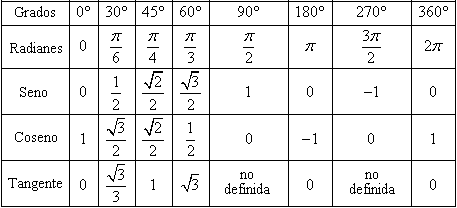
\includegraphics[scale=0.6]{figuras/tablatrig.png}
\end{figure}

\begin{center}
 \subsection{Resultados obtenidos a través del Teorema de De Moivre}
\end{center}

\begin{table}[h]
\begin{center}
\begin{tabular}{| r | l | }
\hline
\rojo{Conjugado: } & $\overline{z} =  r (\cos{(- \theta)} + i \sin{(- \theta)}) = r e^{- \theta i}$\\ \hline
\rojo{Inverso: }   & $z^{-1} =  r^{-1} (\cos{(- \theta)} + i \sin{(- \theta)}) = r^{-1} e^{- \theta i}$\\ \hline
\rojo{Producto: }  & $z \cdot w = r s  (\cos{(\theta + \varphi)} + i \sin{(\theta + \varphi)}) = r s e^{(\theta + \varphi) i}$\\ \hline
\rojo{Cociente: }  & $\frac{z}{w} = \frac{r}{s} (\cos{(\theta - \varphi)} + i \sin{(\theta - \varphi)}) = \frac{r}{s} e^{(\theta - \varphi) i}$\\ \hline
\rojo{Potencias: } & $z^n = r^n (\cos{(n \theta)} + i \sin{(n \theta)}) = r^n e^{ n \theta i}$\\ \hline
\end{tabular}
%\caption{Fruta disponible}
%\label{tab:fruta}
\end{center}
\end{table}

\begin{center}
 \subsection{Raices n-ésimas de un numero $\mathbb{C}$}
\end{center}

\begin{teo} 
$n \in \mathbb{N}$, $z = s e^{i \varphi} \in \mathbb{C}^x$, $s \in \real{}_{>0}$ $\land$ $0 \menig \varphi < 2\pi$ 
$\Rightarrow$ $z$ tiene $n$ raices $w_i \in \mathbb{C}$. Donde: $\left\lbrace \begin{array}{l}
w_k = s^{1/n} e^{{\theta}_k i} \\
{\theta}_k = \frac{\varphi + 2 k \pi}{n}\\
0 \menig k < n
\end{array}\right.$ 
\end{teo}

\begin{center}
\subsection{El Grupo $G_n$ de raices n-ésimas de la Unidad} 
\end{center}

\begin{defi} 
$G_n = \lbrace w \in \mathbb{C} : w^n = 1 \rbrace$ $=$ $\lbrace w_k = e^{\frac{2 \pi k i }{n}} ; 0 \menig k \menig n-1 \rbrace$ $\contenido$ $\mathbb{C}^x$ 
\end{defi}


\begin{prop}
 (($G_n$, $\cdot$) Es grupo Abeliano )
Sea $n \in \mathbb{N}$ $\Rightarrow$ $\left\lbrace \begin{array}{ll}
(1) &  \forall w,z \in G_n \Rightarrow w \cdot z \in G_n\\
(2) & 1 \in G_n\\
(3) & \forall w \in G_n \exists w^{-1} \in G_n
\end{array}\right.$
\end{prop}

\begin{prop}
$n \in \mathbb{N}$ $\land$ $w \in G_n$
\begin{enumerate}
\item $|w| =1$
\item $m \in \mathbb{Z}: n | m \Rightarrow w^m = 1$
\item $m, m' \in \mathbb{Z} / \hspace{0.1cm} m \equiv m' (n) $ $\Rightarrow$ $w^m = w^{m'}$ (En particular, $w^m = w^{r_n(m)}$)
\item $w^{-1} = \overline{w} = w^{n-1}$
\end{enumerate} 
\end{prop}

\begin{prop}
 $\left( G_n \interseccion G_m = G_{(n:m)} \right)$
\begin{enumerate}
\item $n | m$ $\implica$ $G_n \subset G_m$
\item $G_n \interseccion G_m = G_{(n:m)}$ 
\item $G_n \subset G_m$ $\implica$ $n | m$
\end{enumerate}
\end{prop}

\begin{prop} ($G_n$ es ciclico )

$n \in \mathbb{N}$ $\implica$ $\exists w \in G_n$ $/$ $G_n = \lbrace 1,w,w^2, \cdots, w^{n-1}\rbrace$. Notar que no todo $w \in G_n$ cumple dicha consigna. 
\end{prop}



\begin{defi}(Raiz n-ésima primitiva de la unidad)

Sea $n \in \mathbb{N}$. $w \in \mathbb{C}$ es n-esima primitiva de la unidad, $sii$ $G_n = \lbrace 1,w,w^2, \cdots, w^{n-1}\rbrace$ $=$ $\lbrace w^k ; 0 \menig k \menig n-1\rbrace$
\end{defi}
 
\begin{obs}
 $w \in G_n^*$ ($w$ es primitiva) $\implica$ $0 \menig k \cancel{=} j \menig n-1$; $w^k \cancel{=} w^j$, pues $G_n$ tiene $n$ elemnentos distintos y por esto dos potencias de $w$ no pueden coincidir.  
\end{obs}


\begin{propo}
 $w$ es primitiva si $\forall$ $m \in \mathbb{Z}$; $w^m=1$ $\sii$ $n|m$
\end{propo}


\begin{cor}(Raices Primitivas y Potencias)

$n$, $k$ $\in \mathbb{N}$ $\land$ $w \in \mathbb{C}$; $w \in G_n^*$ $\implica$ $w^k$ es primitiva $\sii$ $(n:k) = 1$ 
\end{cor}

\begin{cor}(Raices Primitivas en $G_n$)

$n \in \mathbb{N}$ $\land$ $w_k = e^{\frac{2 k \pi }{n} i }$; $ 0 \menig k \menig n-1$ $\implica$ $w_k \in G_n* \sii (n:k) = 1$
\end{cor}

\begin{cor}
(Raices Primitivas en $G_p$)

$p :=$ primo $\implica$ $k : 1 \menig k \menig p-1$ (es decir, para cualquier $k$ distinto de $0$) $\implica$ $w_k = e^{\frac{2 k \pi }{p} i }$ es primitiva de $G_p$. Es decir, $\forall$ $w \in G_p$; $w \cancel{=} 1$ se tiene que $w$ es p-esima primitiva de la unidad.
\end{cor}

\begin{prop}(Suma y producto de los elementos de $G_n$)

\[n \in \mathbb{N} :
\hspace{0.4cm}
(i) \sum_{w \in G_n}^{} w = 0 
\hspace{0.7cm}
 (ii) \prod_{w \in G_n}^{} w = \left\lbrace \begin{array}{ll}
                                               × 1 & n \hspace{0.1cm} impar \\
                                                 -1 & n \hspace{0.1cm} par
                                              \end{array}\right.\]
\end{prop}
\end{document}
